\chapter{Standard Templates Library}
\section*{17 - Ottobre}
The goal of STL is to represent algorithms in as general form as possible without compromising efficiency.
There is an extensive use of \textbf{templates}, \textbf{overloading} and \textbf{iterators},
which are used for decoupling algorithms from containers,
and can be seen as an abstraction of pointers.\\
STL is very different from the \textit{Java Collection Library} since it does \textbf{not} use \textit{dynamic binding} and is \textbf{not} \textit{object oriented};
instead the STL uses only \textit{static binding} and \textit{inlining}.

\section{Main Entities}
\begin{itemize}
   \item \textbf{Container} collection of \textit{typed} objects
   \item \textbf{Iterator} Generalization of pointer or address;
   used to step through the elements of collections
   \item \textbf{Algorithm} initializing, sorting, searching, and transforming contents of containers
   \item \textbf{Adaptor} Convert from one form to another e.g. iterator from updatable container; or stack from list
   \item \textbf{Function Object} Form of closure (class with "operator()" defined)
   \item \textbf{Allocator} encapsulation of a memory pool
\end{itemize}

\begin{figure}[h]
   \centering
   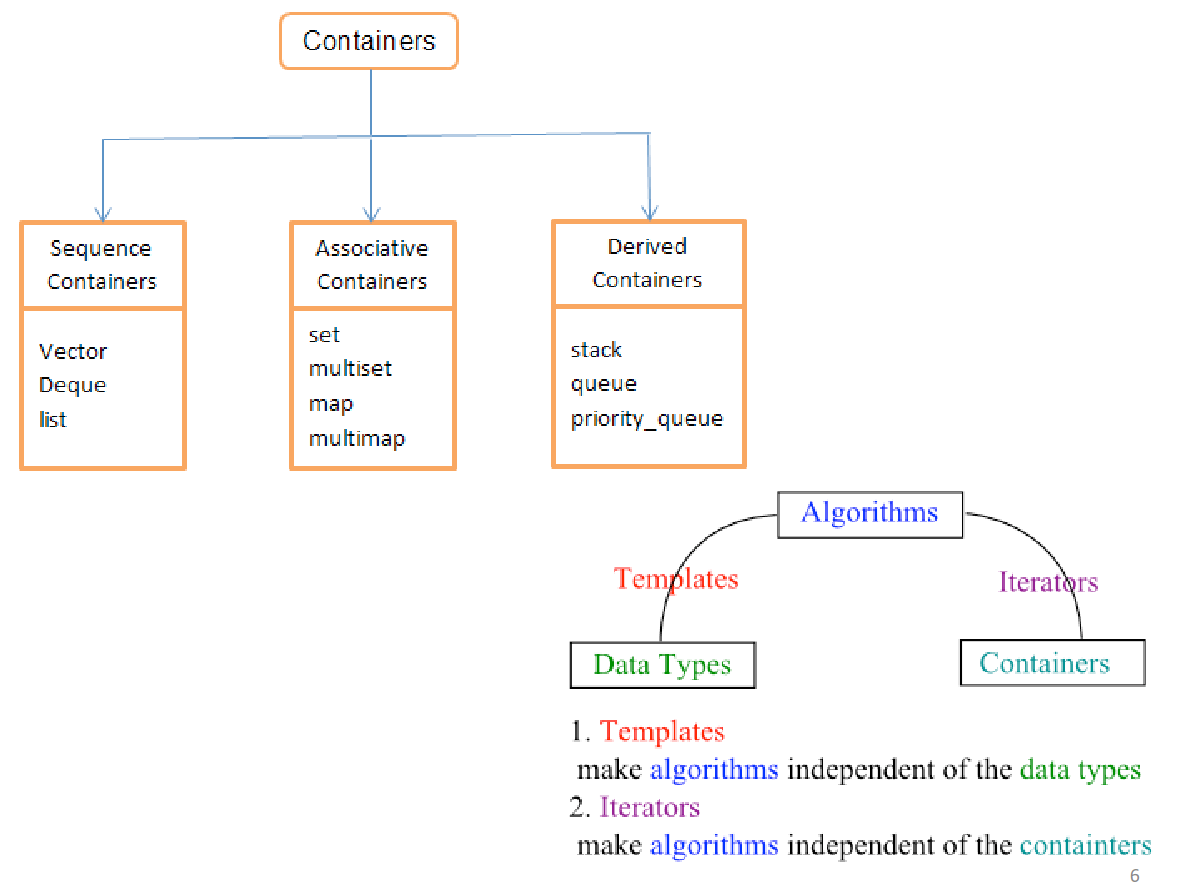
\includegraphics[width=0.7\textwidth]{images/STL_containers.png}
   \label{fig:STL_containers}
   \caption{TIKZ RE-DO : STL Containers}
\end{figure}

\subsection{Iterator}
Since algorithms cannot be used \textit{directly} on different kinds of collections,
Iterators come in handy by providing a \textbf{uniform}, \textbf{linear} access to elements of different collections.

In \textbf{Java} iterators are supported by the \textit{JCF}\footnote{\textit{Java Collection Framework}} through the interface \lstinline|Interface<T>|.
They are related to an \textbf{instance} of a class and are usually defined as \textit{nested classes},
more precisely \textit{non-static private member classes}.\\
Collections equipped with iterators must \lstinline|implements Iterable<T>| interface.